\begin{surferPage}[Labs-Septic]{Septic s 99 singulariteta}
		Oliver Labs je konstruirao plohu stupnja $7$ (septic) dok je radio na svojoj
		disertaciji na Sveu\v cili\v stu u Mainzu, 2004.\ godine. Njegova konstrukcija 
		sa $99$ singulariteta predstavlja trenutni svjetski rekord za plohu stupnja $7$, ali je jo\v s
		uvijek mogu\' ce da postoji ploha septic s najvi\v se $104$ singulariteta.
		Labsova ploha ima simetriju pravilnog sedmerokuta (slika lijevo), \v sto je posebno vidljivo
		kada se na plohu gleda odozgo (slika desno):
		
		\vspace*{-0.3em}
    \begin{center}
      \begin{tabular}{c@{\qquad}c}
        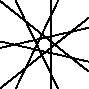
\includegraphics[height=1.5cm]{./../../common/images/labsseptic1.pdf}
        &
        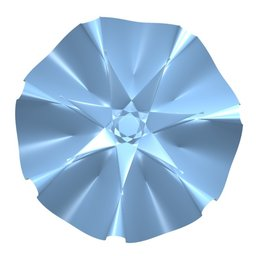
\includegraphics[height=1.5cm]{./../../common/images/labs_septic_von_oben}
      \end{tabular}
    \end{center}
    \vspace*{-0.3em}
		
		Oliver Labs je, kako bi konstruirao ovu plohu, koristio CAS (Computer Algebra System) alat
		{\sc Singular}, koji je prikladan za izra\v cune u algebarskoj geometriji i za singularitete.
		
		Labs je koristio modularnu aritmetiku. Primjer ovoga mo\v zemo prona\' ci u na\v cinu na koji 
		gledamo na sat. Znamo da je 24:00$=$0:00, ali 24:00 $+$ 1 sat nije 25:00 sati, nego 1:00 sat.
\end{surferPage}
